%% LyX 2.3.6.1 created this file.  For more info, see http://www.lyx.org/.
%% Do not edit unless you really know what you are doing.
\documentclass[english]{article}
\usepackage[T1]{fontenc}
\usepackage[latin9]{inputenc}
\setlength{\parskip}{\smallskipamount}
\setlength{\parindent}{0pt}
\usepackage{float}
\usepackage{graphicx}
\usepackage{setspace}
\onehalfspacing
\usepackage{babel}
\begin{document}

\section{Sheath Model}

\subsection{Introduction}

When plasmas with quasi-neutrality ($n_{e}\approx n_{i}$) are joined
to wall surfaces, a positively charged layer called $sheath$ is required
in physics to maintain the balance of electrons and ions. The electron
thermal velcocity $(eT_{e}/m_{e})^{1/2}$ is at least 100 times the
ion thermal velocity $(eT_{i}/m_{i})^{1/2}$, as $T_{e}\ge T_{i}$
and $m_{e}\ll m_{i}$ . Let us assume an initial plasma with zero
electric potenital and E-field everywhere, since $n_{e}=n_{i}$at
$t=0$. The electrons are not confined by any field or potential and
hence move faster to the walls than ions. On a short timescale, some
electrons near the walls are lost, leading to net positive space charges
near the walls. This positively charged space, which is SHEATH, creates
an E-field pointing to the walls, reducing the electron speed and
increasing the ion speed to the walls. Eventually, the loss of electrons
and ions balance each other and plasma remains quasi-neutral. Sheath
plays an important role in the plasma etching. As positive ions flowing
out of the bulk plasma enter the sheath, they get accelerated by the
sheath fields and pick up high energies as they traverse across the
sheath. The ions carry these high energies and delivers to the materials
surface, such as Si surface. The ion etch rates, selectivity and damage
are also impacted by the energies, which are determiend by the sheath.
A diagram of sheath can be seen in the figure below.

Within the Langmuir model, Sheath model serves as a connector between
Reactor model and Feature model. It takes the E-filed and species
from the Reactor model and compute the angular and energy distribution
of electrons and ions, which is fed into the Feature model as input.
Sheath model uses particle tracing algorithm and basically traces
particles under varying E-field. Particle collisions are taken into
account and they widen the distribution of angle. In the code structure,
modules from Feature model, such as particle and move, can be shared
with Sheath model.

\begin{figure}[H]
\begin{centering}
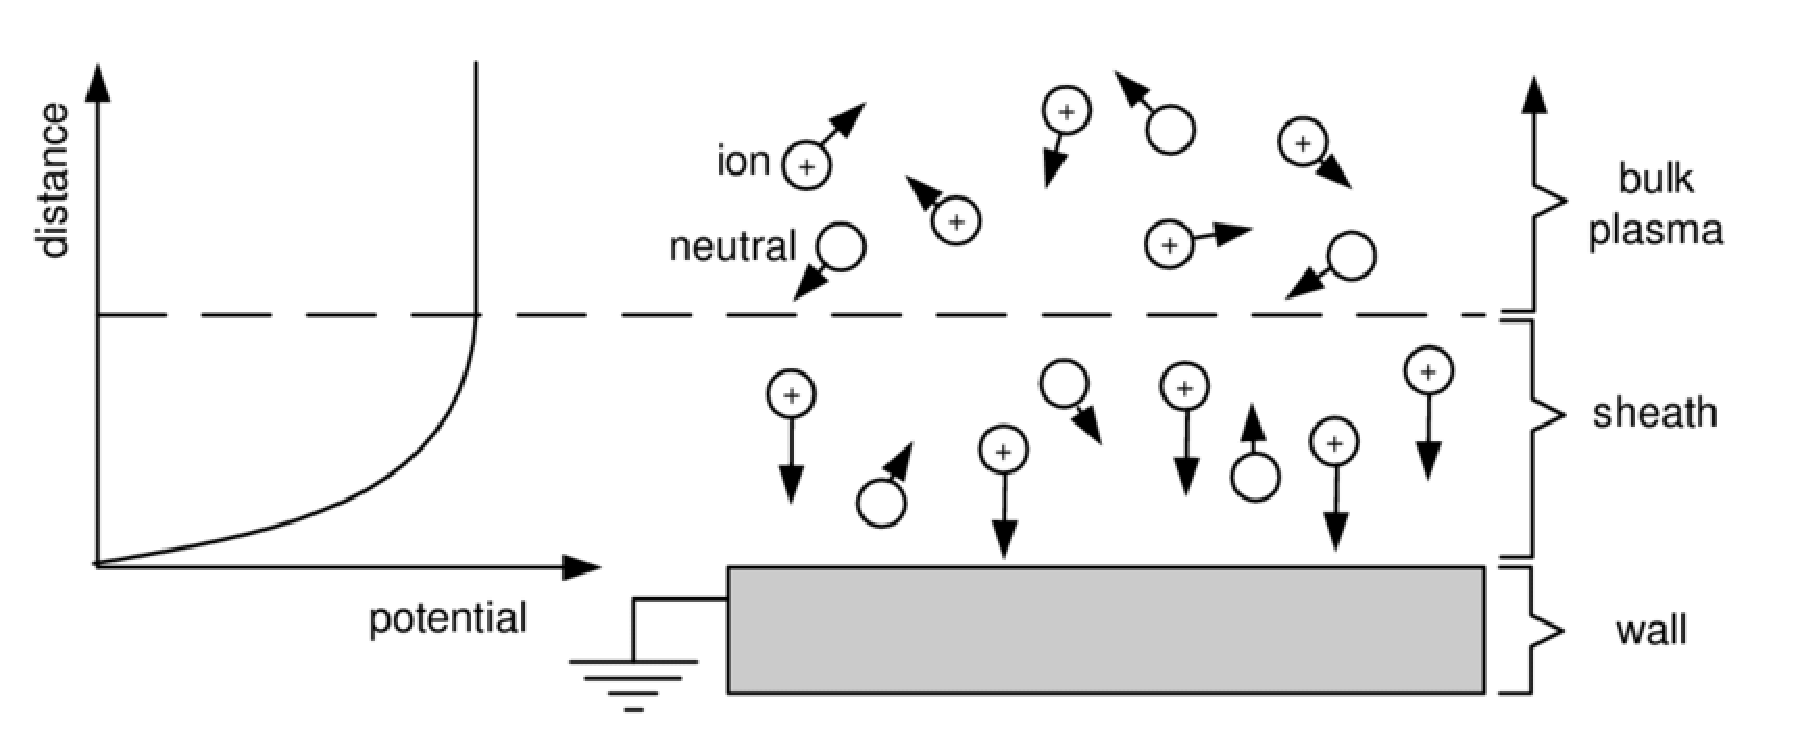
\includegraphics[scale=0.5]{Figures/The-plasma-sheath}
\par\end{centering}
\caption{The plasma sheath. Ions in the plasma happen upon the sheath, where
they are accelerated to the wall. At the wall, ions are neutralized
by electrons from the ground and return to the bulk.}

\end{figure}


\subsection{Collisionless Sheath}

\subsubsection{What is collisionless sheath}

When the ion mean free path is much larger than the sheath thinkness,
the sheath is called a collisionless sheath. Within a collisionless
sheath, the velocites of ions are only determined by the sheath field
and ions are continuously accelerated by the sheath field. Ions pick
up energies as they enter the plasma-sheath edge and exit the sheath
with an energy distribution of a bimodal shape, seen the figure below.
At low frequencies ($\tau_{ion}/\tau_{rf}\ll1$, transverse time of
ion is much smaller than the RF period), the ions traverse the sheath
within a small fraction of an RF cycle. The phase of the RF cycle
at which ions enter the sheath determines their energies at the exit.
In this case, the IED (Ion Energy Distribution) is broad and bimodal,
with the two peaks corresponding to the minimum and maximum of the
sheath drops. At high frequency ($\tau_{ion}/\tau_{rf}\gg1$, transverse
time of ion is much larger than the RF period), it takes the ions
many RF cycles to cross the sheath. In such a scenario, the net energy
gained by the ions is determined by the DC component, which is the
time-averaged sheath voltage. The effect of phase at which they enter
the sheath is significantly reduced. The IED is still bimodal, but
much narrower. 

\begin{figure}[H]
\begin{centering}
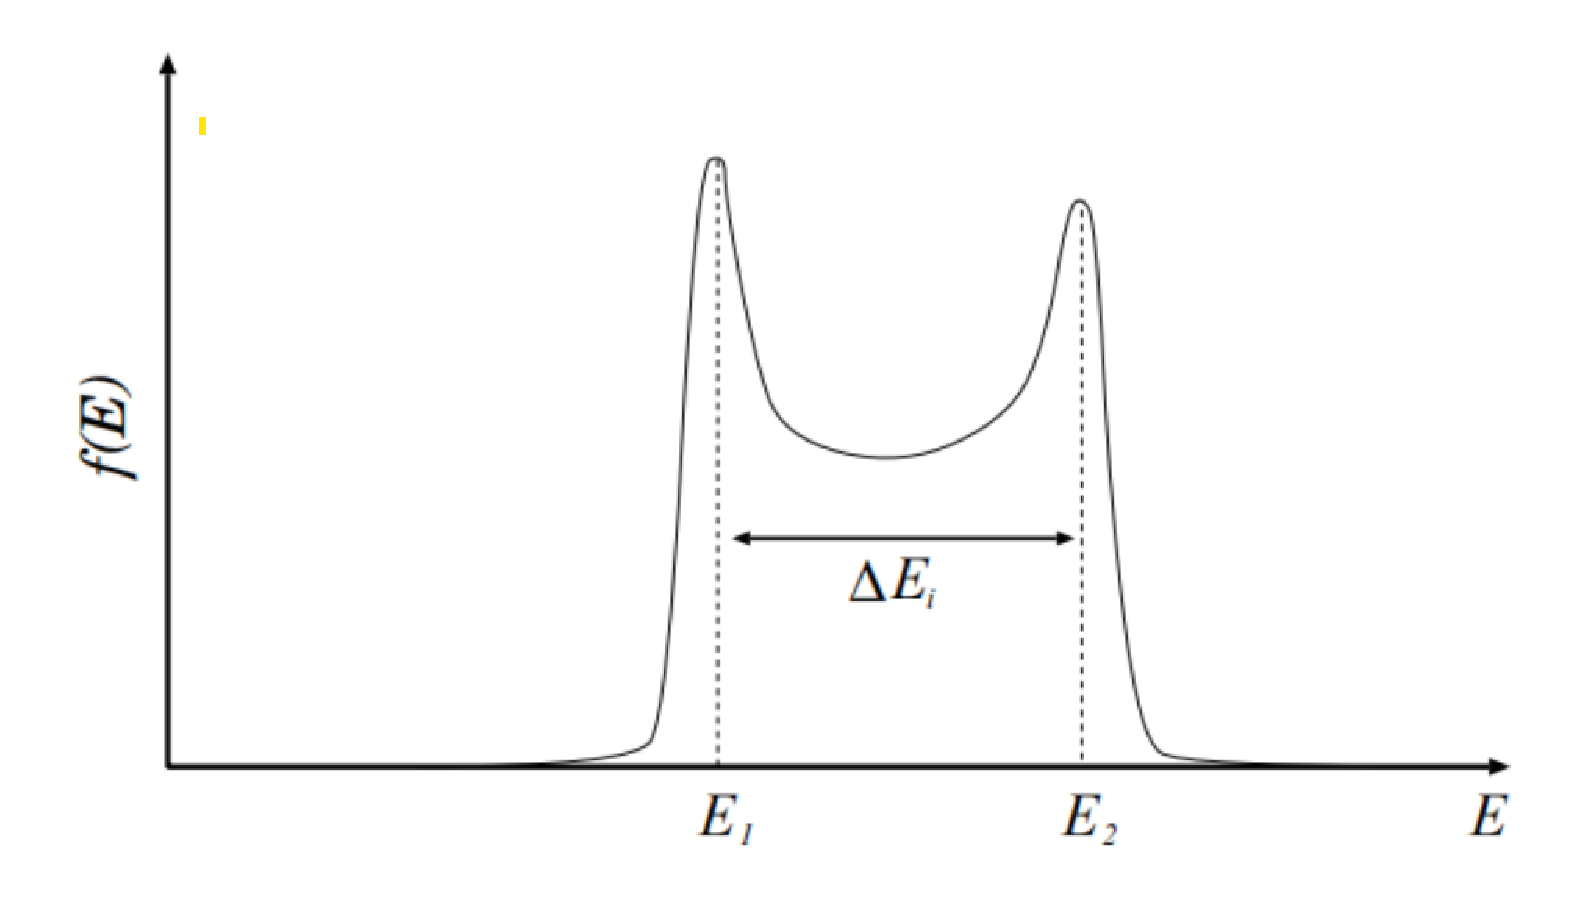
\includegraphics[scale=0.5]{Figures/Bimodal-IED}
\par\end{centering}
\caption{A bimodal ion energy distribution.}

\end{figure}


\subsubsection{Analytic Collisionless Sheath Model}

Benoit-Cattin et al{[}{]} obtained an analytic solution for IED at
the high-frequency regime ($\tau_{ion}/\tau_{rf}\gg1$, transverse
time of ion is much larger than the RF period), assuming 
\begin{enumerate}
\item a constant sheath thickness, $\bar{s}$
\item a uniform sheath electric field, $\vec{E}$is independent of position
$x$ 
\item a sinusoidal sheath voltage $V_{sh}(t)=V_{dc}+V_{s}sin(\omega t)$
\item zero initial ion velocity at the plasma-sheath boundary, $v_{ion}(x=\bar{s})=0$
\end{enumerate}
The resulting expressions for $\Delta E_{i}$and the IED are
\[
\Delta E_{i}=\frac{2eV_{s}}{\bar{s}\omega}(\frac{2eV_{dc}}{m_{i}})^{1/2}=\frac{3eV_{s}}{\pi}(\frac{\tau_{rf}}{\tau_{ion}})
\]
\[
f(E)=\frac{dn}{dE}=\frac{2n_{t}}{\omega\Delta E_{i}}[1-\frac{4}{\Delta E_{i}^{2}}(E-eV_{dc})^{2}]^{-1/2}
\]

where $n_{t}$is the number of ions entering the sheath per unit time.

The calculations yield a bimodal IED with two peaks symmetric about
$eV_{dc}$and $\Delta E_{i}$proportional to $\frac{\tau_{rf}}{\tau_{ion}}$,
seen the figure below.

\begin{figure}[H]
\begin{centering}
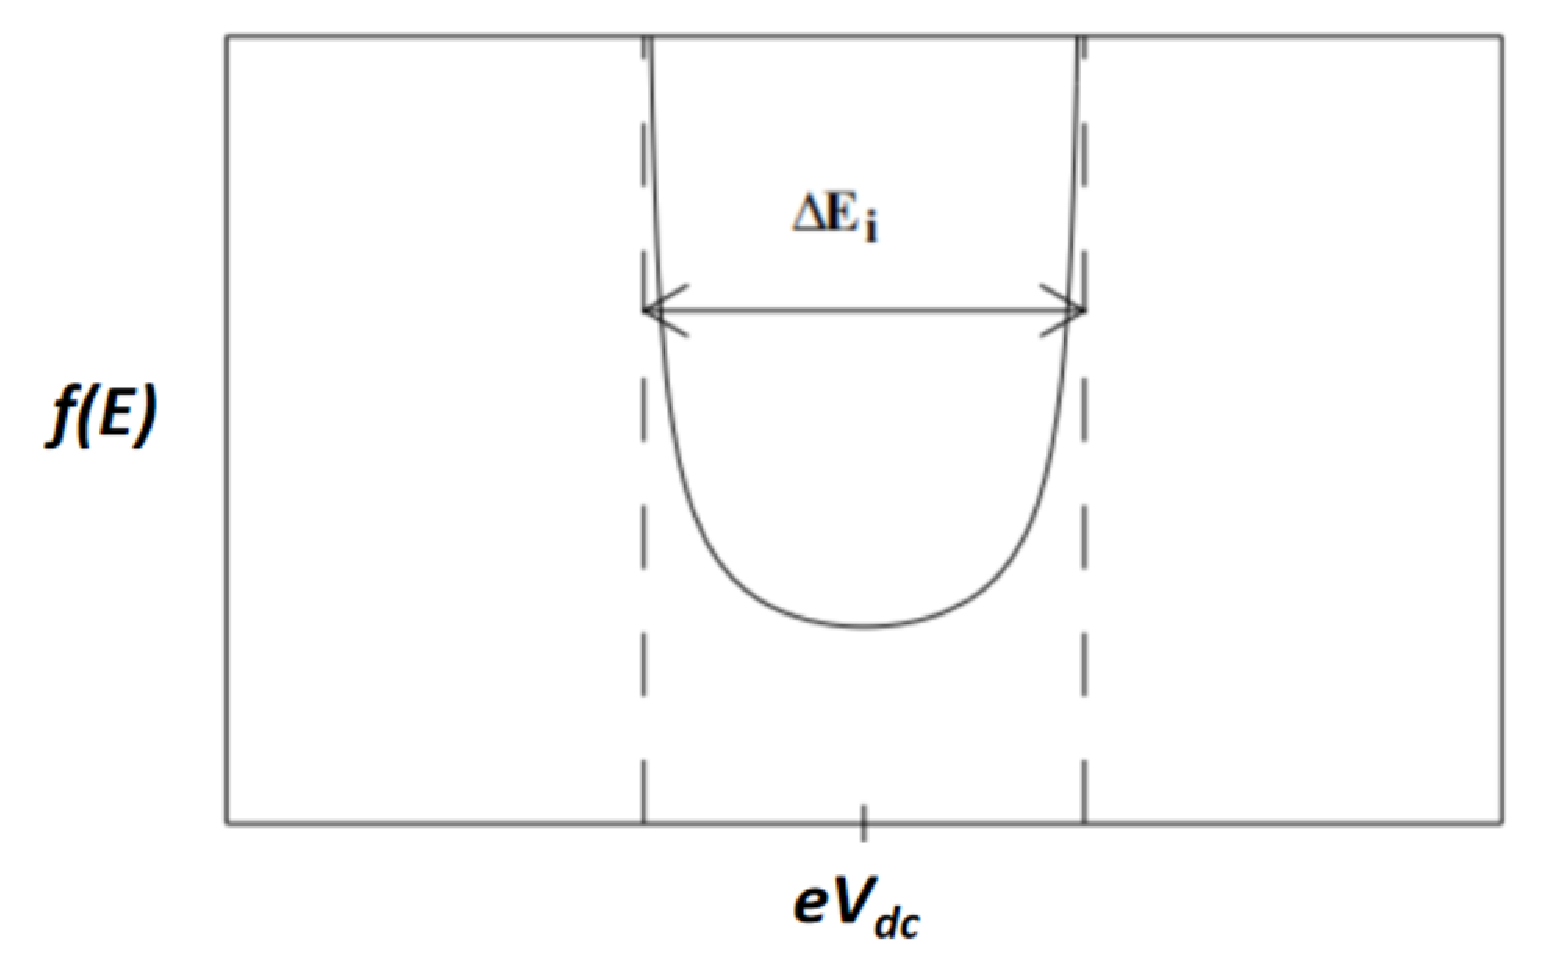
\includegraphics[scale=0.5]{Figures/Bimodal-IED-Analytic}
\par\end{centering}
\caption{The plot of analytic solution for IED at the regime of high frequency
($\tau_{ion}/\tau_{rf}\gg1$) . The singular peaks are due to the
assumption of a mono-energetic initial ion velocity distribution.}
\end{figure}


\subsubsection{Collisionless Sheath Model}

In the collisionless sheath model, we only need to solve the Newton's
euqation, 
\[
\frac{d}{dt}\vec{x}=\vec{v}
\]
\[
\frac{d}{dt}\vec{v}=\frac{eq}{m_{i}}\vec{E}(t)
\]
\[
\vec{E}(\vec{x},t)=f(V_{sh}(x,t),s(t))
\]
\[
\vec{x},\vec{v}-position,velocity
\]
\[
e-elementary\:charge
\]
\[
q-\#\:of\:charges\:carried\:by\:ion
\]
\[
\vec{E}(\vec{x},t)-electric\:field\:within\:sheath
\]
\[
V_{sh}(\vec{x},t)-sheath\:potential
\]
\[
s(t)-sheath\:thickness
\]


\subsection{Collisional Sheath}

When the mean free path of ions, $\lambda_{ion}$, is much smaller
than the sheath thickness, the ions entering the sheath will experience
collisions before exit. Collisions can alter the velocity, both speed
and angle. Since the ion density is much smaller than background neutral
density within the sheath, ion-neutral collisions dominate the ion
collisions. In the sheath model, there is no ion-ion collisions, or
even interactions. In another word, ions are independent from each
other. The probability of a collision event occurring depends on the
ion-neutral collision frequency, $v_{in}$, which is defined as:
\[
v_{in}=N_{d}\sigma|\vec{v}_{i}-\vec{v}_{g}|
\]
\[
N_{d}-backgroud\:number\:density\;(m^{-3})
\]
\[
\sigma-ion-neutral\:charge\:exchange\:collision\:cross\:section\;(m^{2})
\]
\[
\vec{v}_{i},\vec{v}_{g}-ion\:velocity,\:background\:gas\:velocity\;(m/s)
\]

The collision probability defined as 
\[
P=1-exp(-v_{in}\Delta t)=1-exp(-\frac{\Delta x}{\lambda_{ion}})
\]

If a collision occurs, the particle velocity is updated according
to following expression:
\[
\vec{v}_{i}^{'}=\frac{m_{i}\vec{v}_{i}+m_{g}\vec{v}_{g}-m_{g}|\vec{v}_{i}-\vec{v}_{g}|\vec{U}}{m_{i}+m_{g}}
\]
\[
\vec{v}_{i}^{'}-after-collision\:ion\:velocity
\]
\[
m_{i},m_{g}-mass\:of\:ion,\:background\:gas
\]
\[
\vec{U}-a\:uniformly\:distributed\:random\:unit\:vector
\]

in the equation above, $\vec{v}_{g}$ is sampled from a Maxwellian
distribution function, assuming the background neutral gas is in thermal
equilibrium state.

\subsection{Analytic Sheath Model}
\end{document}
